
\section{Methodology}

\subsection{Research Design}
Given the potential for memory bias due to the passage of time since the project's inception, this study employs a mixed-methods approach. While human memory can be fallible, introducing biases and even constructing false memories, quantitative analysis serves as a foundational component to mitigate these challenges. It allows for the identification of key contributors based on metrics such as commit frequency and significance, forum participation, and library contributions. These quantitative findings inform the selection of interviewees, acting as a preliminary filter to locate core contributors and library authors for qualitative interviews.

% todo NN attention : tu cites ici une généralité sans référence…
Anthropological studies have consistently highlighted the limitations of relying solely on quantitative data to understand the complex interplay of human experiences, beliefs, and emotions. Hence, qualitative interviews stand as a cardinal ethnographic instrument, offering access to the lived experiences, emic perspectives, and personal narratives of participants—dimensions that are often obscured in purely numerical representations.

By purposefully integrating quantitative methodologies with qualitative ethnographic approaches, this research aspires to offer a nuanced understanding of both the structural and phenomenological aspects of the Processing community.

\subsection{Quantitative Methods}
\subsubsection*{Data sources}

The research draws upon multiple data sources to form a comprehensive picture of the Processing community and its development practices. These range from forum discussions at various phases of the project to commit histories and issue trackers. The parsing status indicates the extent to which each data source has been prepared for analysis. 
\begin{table}[h]
    \raggedright
    \caption{Data sources}
    \label{table:data-sources}
    \begin{tabular}{l l l c}
        \toprule
        Name & Type & Status \\
        \midrule
        Processing alpha forum & Forum & Parsed \\
        Processing beta forum & Forum & Parsed  \\
        Processing 1.0 forum & Forum & Downloaded \\
        Processing 2.0 and 3.0 forum & Forum  & Not downloaded \\
        Current processing forum & Forum & Not downloaded\\
        Github project & Commit history & Parsed \\
        Processing Release Data & Release notes & Parsed \\
        Github Release Data & Release notes \& download statistics & Parsed \\
        Processing libraries\textsuperscript{*} & Software release information & Parsed \\

        \bottomrule
        \multicolumn{3}{l}{\footnotesize \textsuperscript{*}Note: The data set was reconstructed from the processing website archive and is not complete.}
    \end{tabular}
  \end{table}        

\subsubsection*{Evolution of Community Discussion Platforms}
In the early days of the Processing project, community interactions predominantly took place on forums. These forums served as a primary channel for users to share experiences, discuss problems, and seek help. Notably, the forum discussions underwent significant transformations in terms of platforms over the years, as can be observed in Table \ref{table:forums}. \parencite{ProcessingForum}

\begin{table}[h]
    \raggedright
    \caption{Archival forums composition}
    \label{table:forums}
    \begin{tabular}{l l l c}
        \toprule
        Forum name & Years & URL \\
        \midrule
        Processing alpha forum & 2002-2005 & \href{https://forum.processing.org/alpha/}{forum.processing.org/alpha} \\
        Processing beta forum & 2005-2010 & \href{https://forum.processing.org/beta/}{forum.processing.org/beta}  \\
        Processing 1.0 forum & 2010-2013 & \href{https://forum.processing.org/one/}{forum.processing.org/one} \\
        Processing 2.0 and 3.0 forum & 2013-2018 & \href{https://forum.processing.org/two/}{forum.processing.org/two} \\
        Current processing forum & 2018 - now & \href{https://discourse.processing.org/}{discourse.processing.org} \\
        \bottomrule
    \end{tabular}
  \end{table}

This dynamic shift from one platform to another indicates an evolving user-base and a growing set of needs and tools that community members require for effective collaboration.

\subsubsection*{Shift in Software-Related Discussions}

Initially, software-related discussions were confined to these forums. However, as the project matured, the complexity of issues warranted more specialized platforms for effective tracking and resolution. Consequently, the community transitioned from forums to Bugzilla \parencite{BugzillaArchiveProcessing} and eventually to GitHub Issues\parencite{ProcessingProcessingSource}\parencite{ProcessingProcessing4Processing}. 

\subsubsection*{The Ecosystem of Libraries}
An important milestone in the Processing ecosystem was the introduction of libraries. These libraries extended the functionalities of the base platform, thereby attracting a broader range of users and contributors. Such an analysis not only sheds light on the diversification of the project but also identifies key contributors and library authors who could potentially be sought out for qualitative interviews. The identification of these contributors adds another layer to our understanding of community participation.

\newpage
This is a page to test the script

\changepapersize{305.3mm:210mm}
\customtag{largepage}

\begin{figure}[h!] 
    \centering 
    \includesvg[pretex=\sffamily\fontsize{5.58pt}{8pt}\selectfont, width=1\textwidth, keepaspectratio]{images/figure-libraries.svg}
    \caption{Distribution of Libraries in the Processing Project}
    \label{figure:libraries}  
  \end{figure}

\defaultareasettings

% todo NN ce serait bien de mieux valoriser cette figure 2 visuellement, dans une mise en page aérée et large


% todo add
%\subsubsection{Forum Textual Analysis: Approach and Tools}
%The research process began by manually reading the forum to identify themes and complemented with quantitative approaches. 
%todo forum composition





% \begin{figure}[h] 
%   \centering 
%   \includegraphics[width=1\textwidth]{} 
%   \caption[Ben Fry at PCD 2018]{Ben Fry with conference attendees. Source: \citefield{guptaBenFryConference2018}{author}, Medium, \citeyear{guptaBenFryConference2018}.}

%   \label{figure:benfry-pcd}  
% \end{figure}
% \textbf{Note.} Source: \textcite{guptaBenFryConference2018}.

\subsection{Qualitative Methods}
\begin{figure}[H]
  \begin{minipage}{\textwidth}
    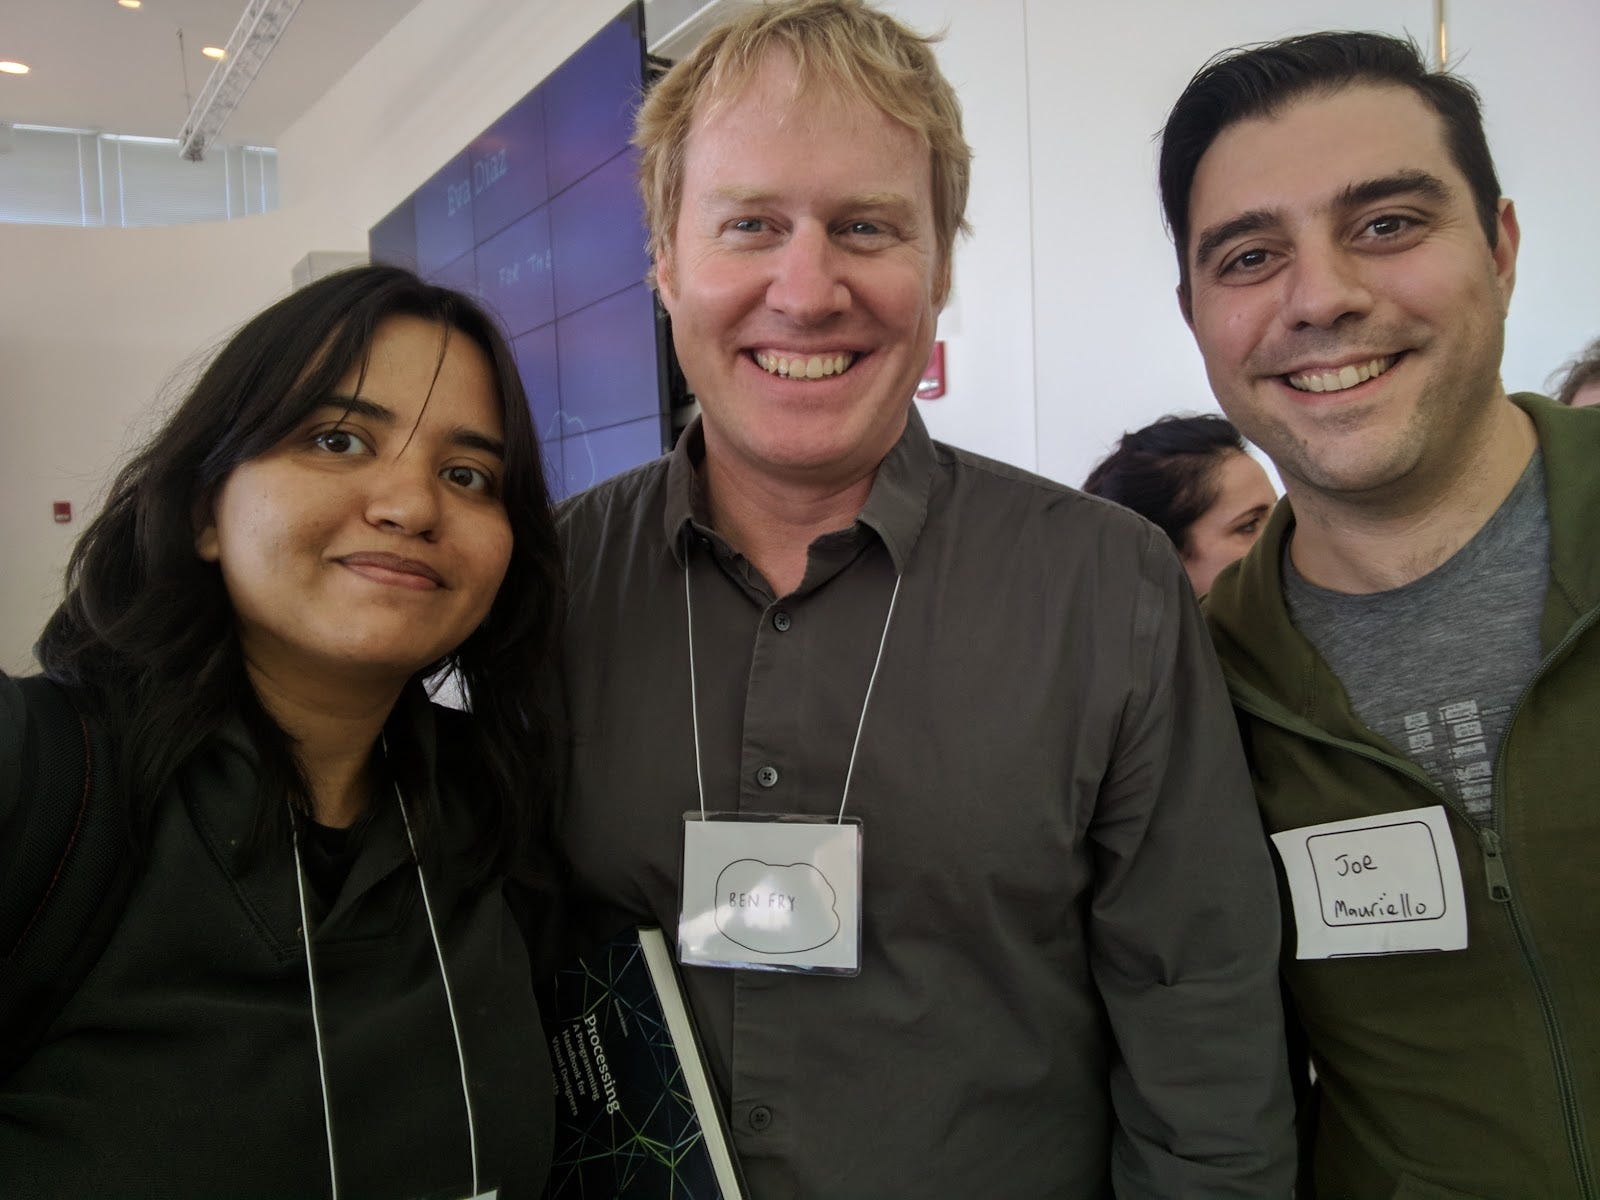
\includegraphics[width=\linewidth]{images/pcd2018.jpg}
    \caption[Ben Fry at PCD 2018]{Ben Fry with conference atendees at Processing Community Day 2018. \fullcitefigure{guptaBenFryConference2018}.}
    \label{fig:benFry}
    
  \end{minipage}
\end{figure}

For this study, the primary qualitative method utilized is semi-structured interviews. This choice was driven by the need for a flexible yet organized approach to gather in-depth insights from participants.

The selection of interviewees was strategically informed by the results of quantitative analyses, particularly in areas where abundant data was available. This methodological triangulation enhances the reliability and depth of the findings.

Interviewees were mainly categorized into distinct populations, which are as follows:

\begin{itemize}
    \item Individuals with the highest number of git commits during the period of the alpha forum, from August 2, 2002, to April 19, 2005.
    \item Members who exhibited the most significant activity on the alpha forum within the same time frame.
    \item Authors of libraries with the most frequent release activity, based on available data spanning from October 26, 2011, to June 8, 2014.
\end{itemize}

Although the Processing Foundation was formalized subsequent to the period under study, it was deemed necessary to include its founding board members in the pool of interviewees. The foundation project’s mission started as the promotion of software and visual literacy through making the development of the core API, and Processing Development Environment (PDE) sustainable. Therefore, its influence is integral to the present investigation.\parencite{robertsProcessingFoundationForm2013}

There are also noteworthy contributors to the Processing ecosystem that fall outside the scope of this paper. These include:

\begin{itemize}
    \item Individuals engaged in writing documentation, examples, and books.
    \item Those participating in or organizing local Processing Community Days or other community events.
    \item Google Summer of Code participants and mentors.
    \item Recipients of fellowship programs.
\end{itemize}

\subsection{The Role of the Processing Foundation}

The Processing Foundation was established in 2012 by Casey Reas, Ben Fry, and Daniel Shiffman with the primary objective of sustaining the software's development and broadening its reach. According to Fry and Reas, ``The vast majority of the code is written by the same small number of people volunteering their time — there are no paid full-time developers'' \parencite[p.~13]{fryModernPrometheusHistory2018}.

\begin{figure}[h]
    \centering
    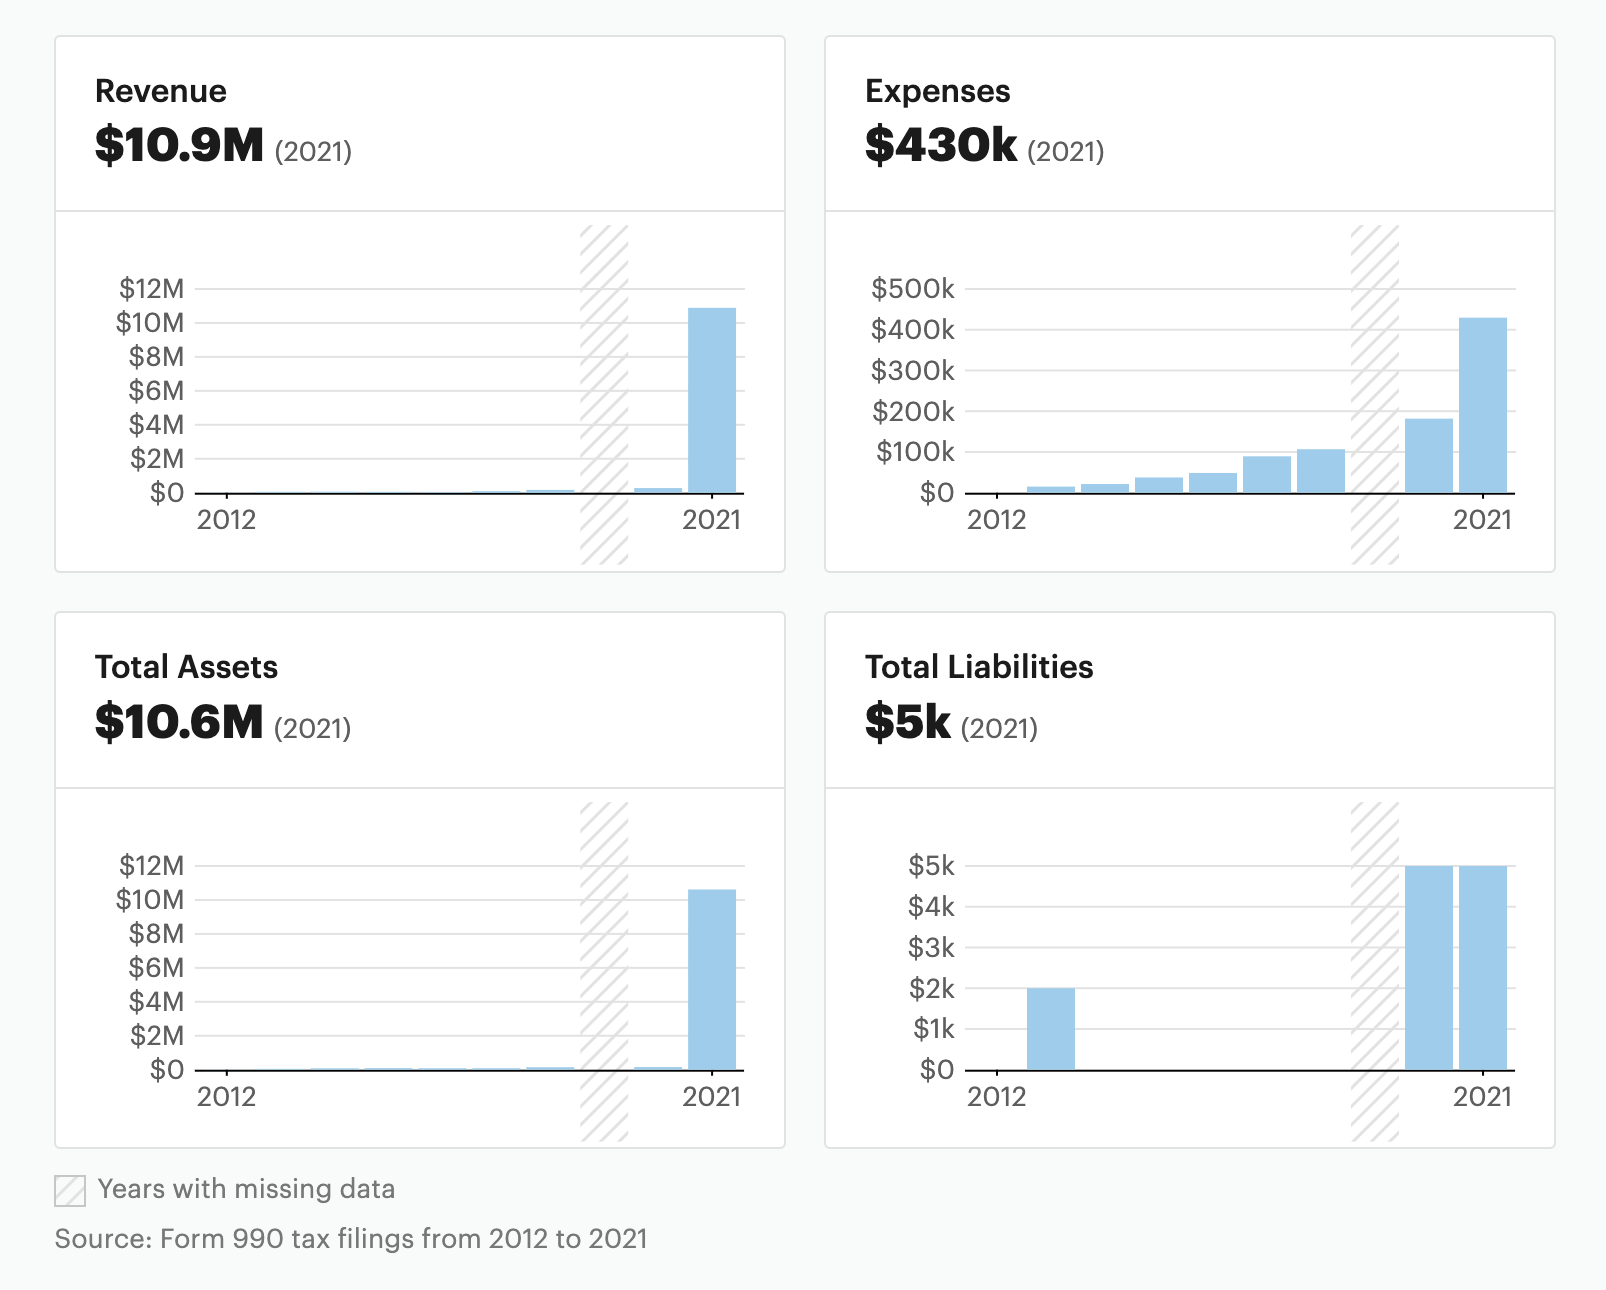
\includegraphics[width=0.9\textwidth]{images/foundation-finances.png} 
    \caption{Financial growth of the Processing Foundation over the years Source: \parencite{ProcessingFoundationNonprofit2013}}
    \label{fig:foundation-finances}
\end{figure}

As shown in Figure~\ref{fig:foundation-finances}, the foundation's revenue has experienced modest growth, increasing from \$11,235 to \$273,520. Remarkably, it reached a peak revenue of \$10,889,998 in the fiscal year 2021. Throughout its history, the principal source of funding for the foundation has predominantly come from contributions. 

However, the allocation of these funds has been a point of contention within the organization. Most notably, a public disagreement in 2023 led to the resignation of Ben Fry, a long-standing board member and contributor. It should be noted that Fry's perspective on the matter was not universally accepted among the foundation's other founding members. \parencite{benfry[@ben_fry]HaveMadeExtremely2023} \parencite{caseyreas[@reas]EarlierThisWeek2023} \parencite{danielshiffman[@shiffman]WouldPostNote2023}
